\documentclass{article}
\title{Homework5.2}
\author{Blue}
\date{20230316}
\usepackage{geometry}
\geometry{a4paper,scale=0.8}
\usepackage{graphicx}
\usepackage{float}
\usepackage{indentfirst}
\usepackage[namelimits]{amsmath} %数学公式
\usepackage{amssymb}             %数学公式
\usepackage{color}
\usepackage{longtable}
\usepackage{listings}
\lstset{
language=Matlab,
numbers=left,
keywordstyle=\color{blue},
numberstyle=\tiny,
breaklines=true,
extendedchars=flase
}
\begin{document}
\maketitle
\section{Question a}
We plot the simulation together with the ode45 solution in section (c).


\section{Question b}
\begin{align}
&\frac{da}{dt}=-2k_1a^2-k_2ab+k_3\\
&\frac{db}{dt}=-k_2ab+k_4
\end{align}
The function assume that 4 reactions happen every moment.$\frac{da}{dt}$ and $\frac{db}{dt}$ describe the changing rate of molecule a and b. As for molecule a, process 1 consume 2 molecules at rate $k_1$. Process 2 consume 1 molecules at rate $k_2$. Process 3 generate molecule at rate $k_3$. As for molecule b, process 2 consume 1 molecule at rate $k_2$, Process 4 generate molecules at rate $k_4$. Therefore the function accurately describe the chemical system above.\\
Apply (10,10) to the function and get:
\begin{align}
&\frac{da}{dt}=-2*10^{-3}*10^{2}-10^{-2}*10*10+1.2=0\\
&\frac{db}{dt}=-10^{-2}*10*10+1=0.
\end{align}
Therefore, (10,10) is a fixed point of this system.
\section{Question c}
We simulate 500 and 1000 chemical reactions of the system and plot them together in the graph. It seems that the deterministic equations converge to the steady state after a number of reactions. In the stochastic process, the number of molecules A and B rises to the steady states and then oscillates around the it.


\begin{figure}[htbp]
    \centering
    \begin{minipage}{0.45\linewidth}
        \centering
        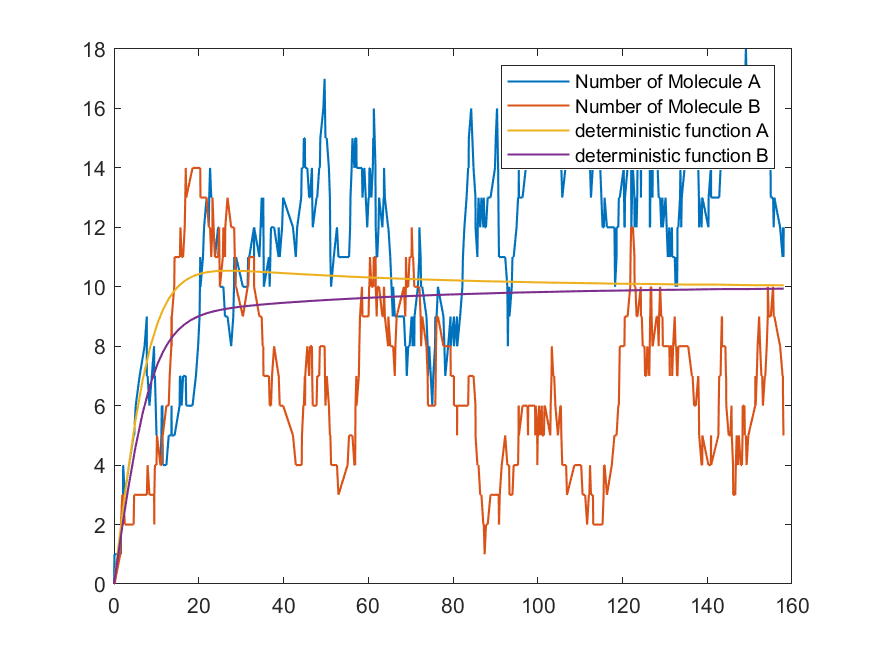
\includegraphics[width=\linewidth]{graph/a1.png}
        \caption{500Simulation1}
        \label{a1}
    \end{minipage}
    \hfill
    \begin{minipage}{0.45\linewidth}
        \centering
        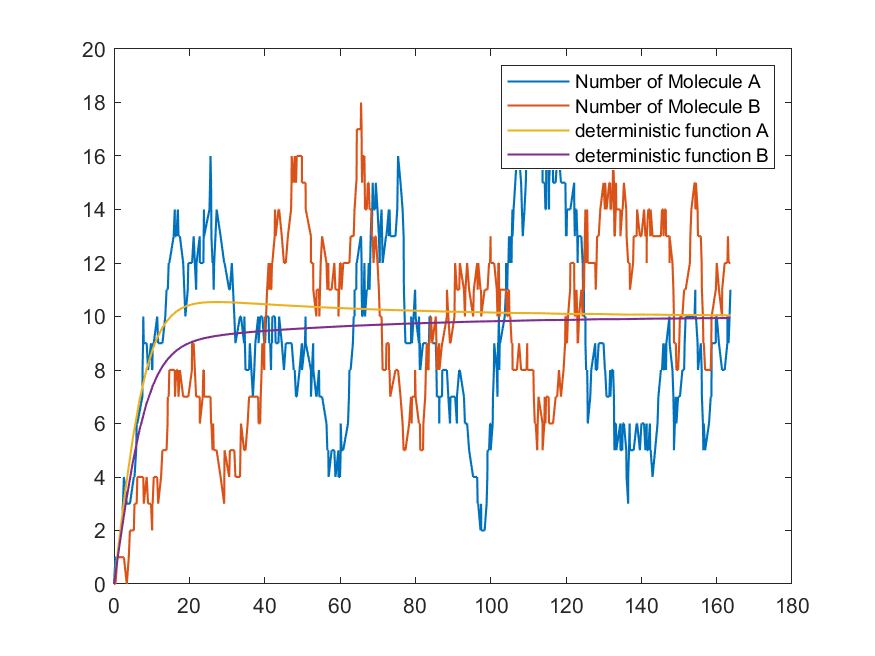
\includegraphics[width=\linewidth]{graph/a2.png}
        \caption{500Simulation2}
        \label{a2}
    \end{minipage}
\end{figure}
\begin{figure}[htbp]
    \centering
    \begin{minipage}{0.45\linewidth}
        \centering
        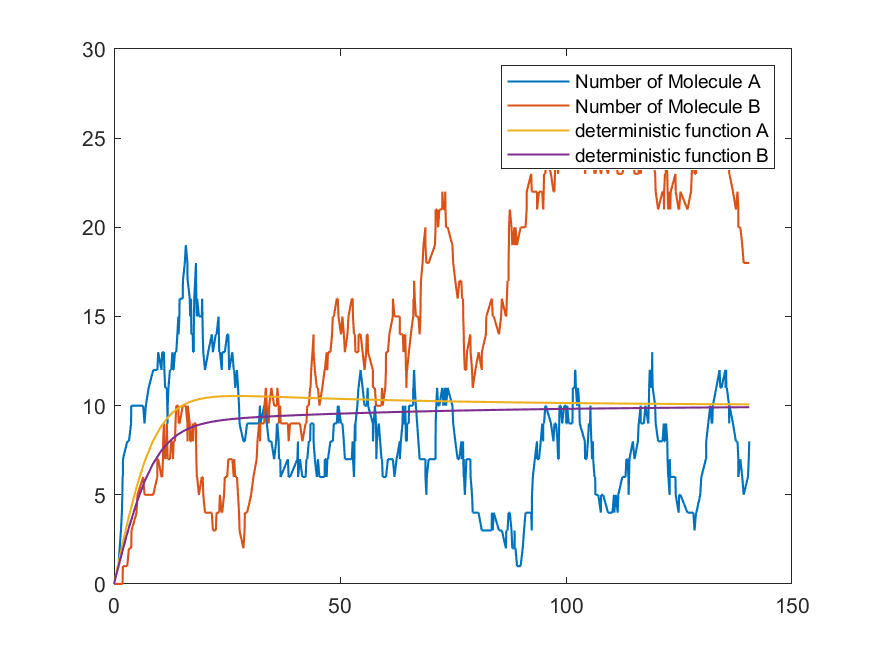
\includegraphics[width=\linewidth]{graph/a3.png}
        \caption{500Simulation3}
        \label{a3}
    \end{minipage}
    \hfill
    \begin{minipage}{0.45\linewidth}
        \centering
        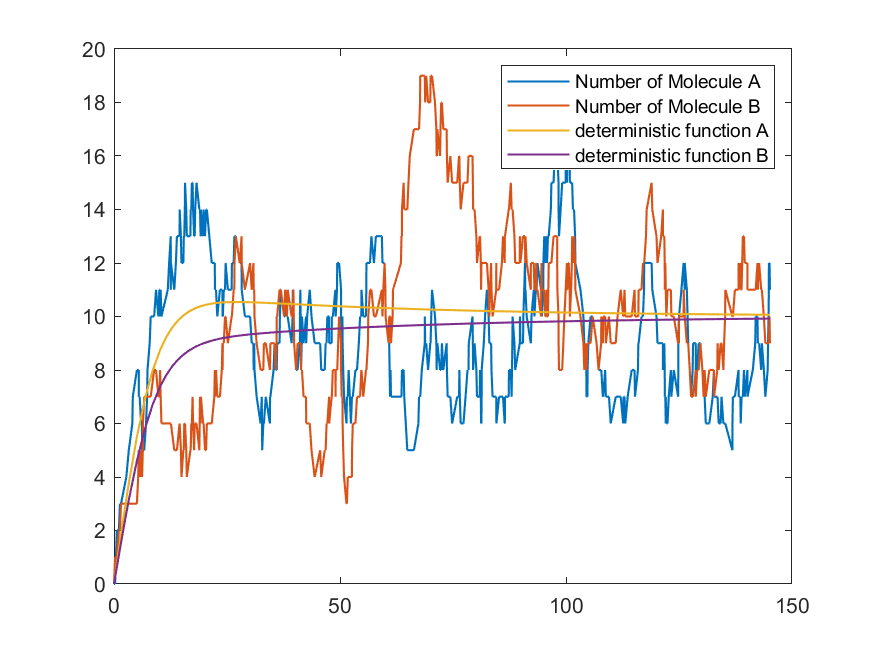
\includegraphics[width=\linewidth]{graph/a4.png}
        \caption{500Simulation4}
        \label{a4}
    \end{minipage}
\end{figure}
\begin{figure}[htbp]
    \centering
    \begin{minipage}{0.45\linewidth}
        \centering
        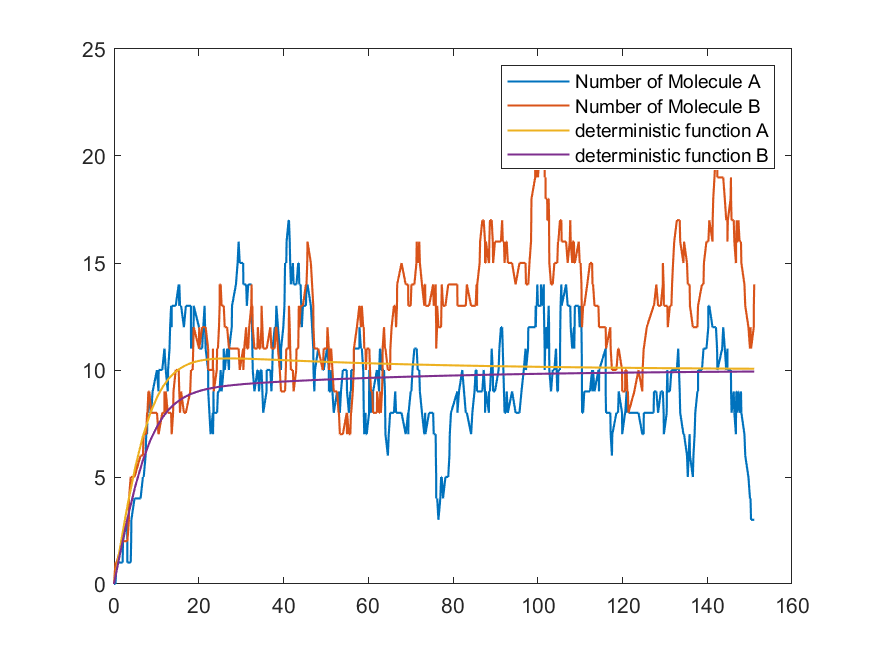
\includegraphics[width=\linewidth]{graph/a5.png}
        \caption{500Simulation5}
        \label{a5}
    \end{minipage}
    \hfill
    \begin{minipage}{0.45\linewidth}
        \centering
        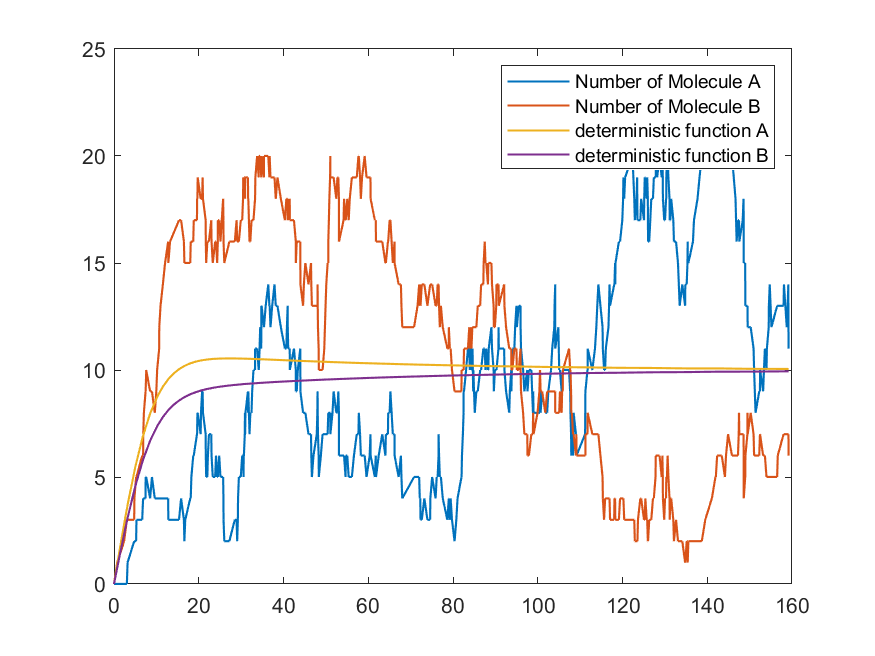
\includegraphics[width=\linewidth]{graph/a6.png}
        \caption{500Simulation6}
        \label{a6}
    \end{minipage}
\end{figure}


\begin{figure}[htbp]
    \centering
    \begin{minipage}{0.45\linewidth}
        \centering
        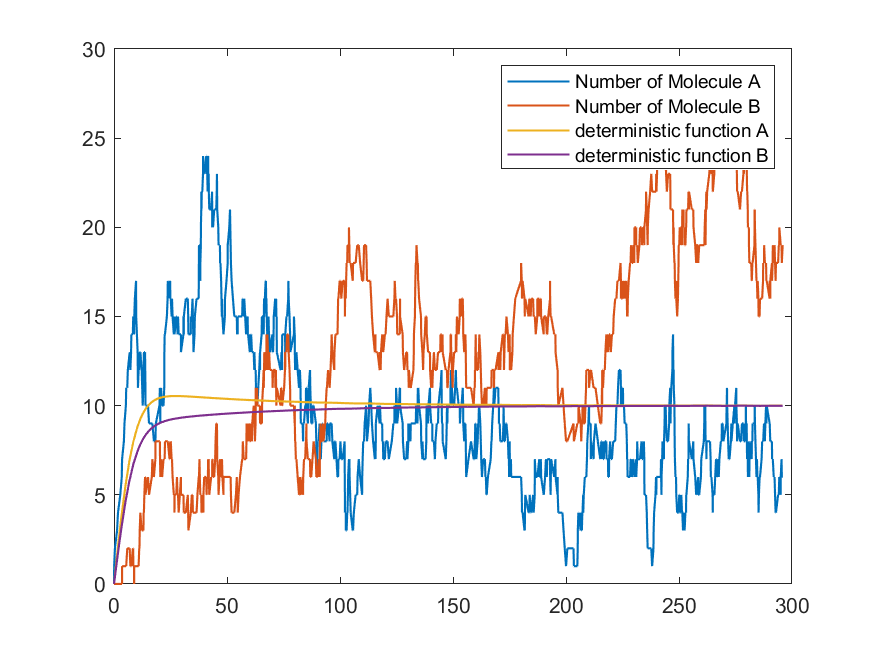
\includegraphics[width=\linewidth]{graph/b1.png}
        \caption{1000Simulation1}
        \label{b1}
    \end{minipage}
    \hfill
    \begin{minipage}{0.45\linewidth}
        \centering
        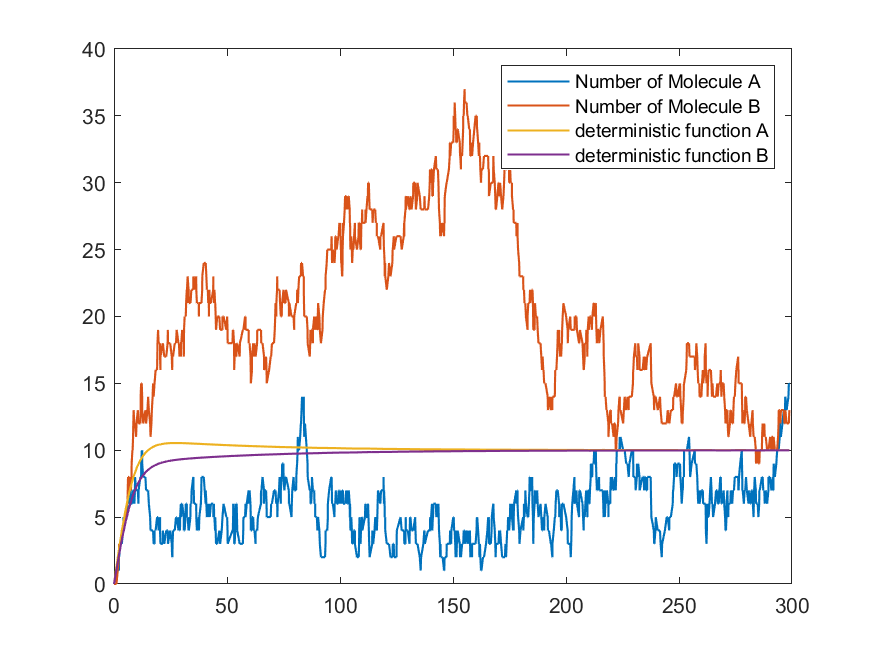
\includegraphics[width=\linewidth]{graph/b2.png}
        \caption{1000Simulation2}
        \label{b2}
    \end{minipage}
\end{figure}
\begin{figure}[htbp]
    \centering
    \begin{minipage}{0.45\linewidth}
        \centering
        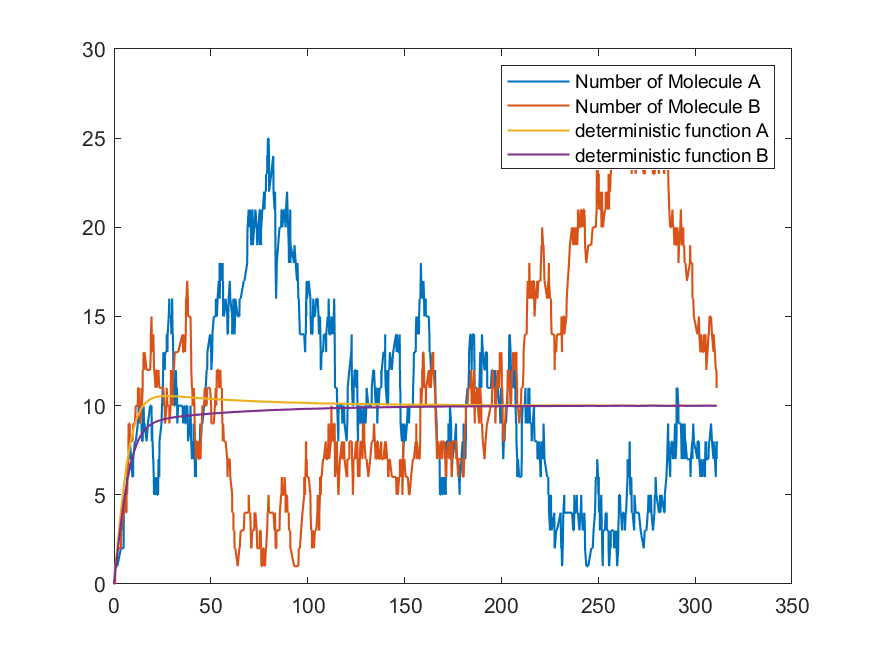
\includegraphics[width=\linewidth]{graph/b3.png}
        \caption{1000Simulation3}
        \label{b3}
    \end{minipage}
    \hfill
    \begin{minipage}{0.45\linewidth}
        \centering
        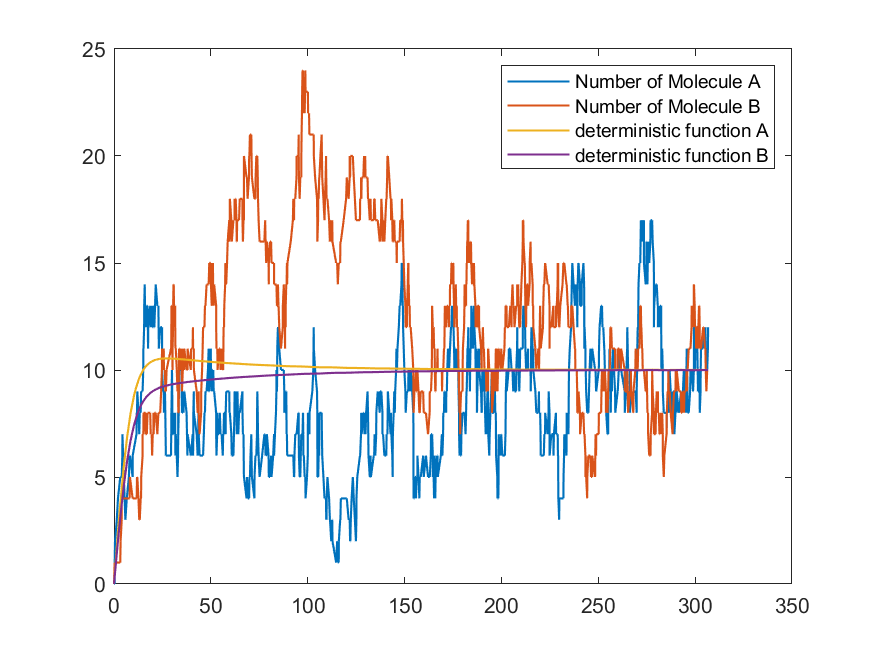
\includegraphics[width=\linewidth]{graph/b4.png}
        \caption{1000Simulation4}
        \label{b4}
    \end{minipage}
\end{figure}
\begin{figure}[htbp]
    \centering
    \begin{minipage}{0.45\linewidth}
        \centering
        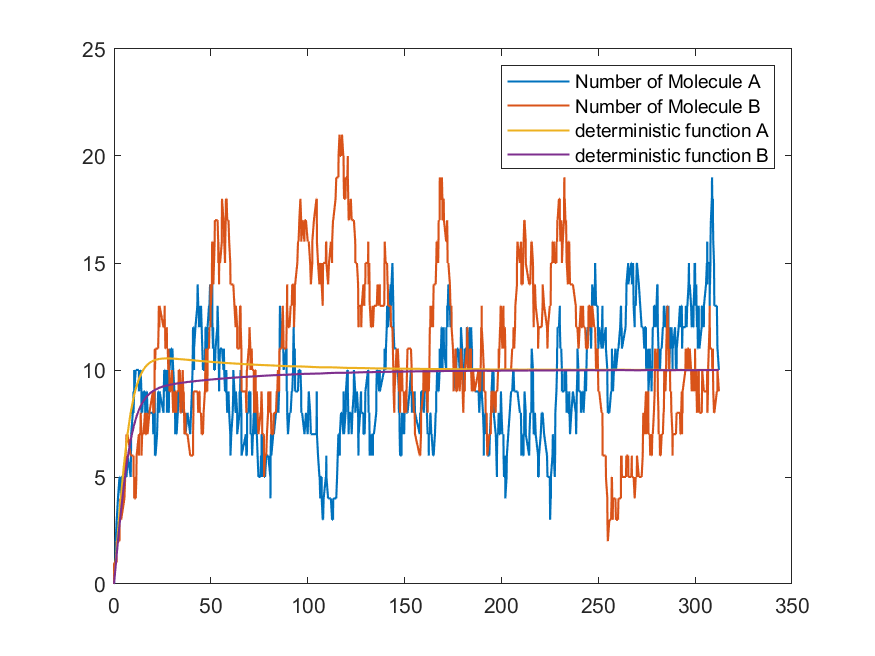
\includegraphics[width=\linewidth]{graph/b5.png}
        \caption{1000Simulation5}
        \label{b5}
    \end{minipage}
    \hfill
    \begin{minipage}{0.45\linewidth}
        \centering
        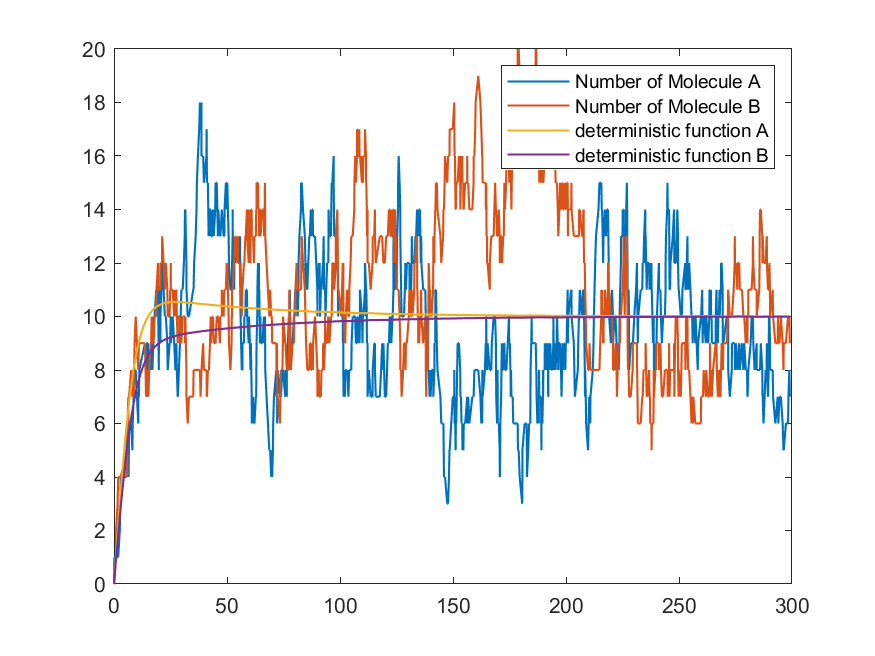
\includegraphics[width=\linewidth]{graph/b6.png}
        \caption{1000Simulation6}
        \label{b6}
    \end{minipage}
\end{figure}

\clearpage









\section{code}
\subsection{Comparison}
\begin{lstlisting}
k1=0.001;
k2=0.01;
k3=1.2;
k4=1;
a0=0;
b0=0;
gillespie2(500,k1,k2,k3,k4,a0,b0,'a1.png');
gillespie2(500,k1,k2,k3,k4,a0,b0,'a2.png');
gillespie2(500,k1,k2,k3,k4,a0,b0,'a3.png');
gillespie2(500,k1,k2,k3,k4,a0,b0,'a4.png');
gillespie2(500,k1,k2,k3,k4,a0,b0,'a5.png');
gillespie2(500,k1,k2,k3,k4,a0,b0,'a6.png');
gillespie2(1000,k1,k2,k3,k4,a0,b0,'b1.png');
gillespie2(1000,k1,k2,k3,k4,a0,b0,'b2.png');
gillespie2(1000,k1,k2,k3,k4,a0,b0,'b3.png');
gillespie2(1000,k1,k2,k3,k4,a0,b0,'b4.png');
gillespie2(1000,k1,k2,k3,k4,a0,b0,'b5.png');
gillespie2(1000,k1,k2,k3,k4,a0,b0,'b6.png');
function gillespie2(m,k1,k2,k3,k4,a0,b0,name)
M=m;
T=zeros(M+1,1);
A=zeros(M+1,1);
B=zeros(M+1,1);
t=0;
A(1)=a0;
B(1)=b0;
a=a0;
b=b0;
for i=2:M+1
    r1=rand;
    r2=rand;
    alpha1=a*(a-1)*k1;
    alpha2=b*a*k2;
    alpha3=k3;
    alpha4=k4;
    alpha=alpha1+alpha2+alpha3+alpha4;
    t=t+log(1/r1)/(alpha);
    if r2<alpha1/alpha
        a=a-2;
    elseif r2<(alpha1+alpha2)/alpha
        a=a-1;
        b=b-1;
    elseif r2<(alpha1+alpha2+alpha3)/alpha
        a=a+1;
    else 
        b=b+1;
    end
    A(i)=a;
    B(i)=b;
    T(i)=t;
end
plot(T,A, 'LineWidth', 1,'DisplayName', 'Number of Molecule A');hold on
plot(T,B,'lineWIdth',1,'DisplayName','Number of Molecule B');
[T2,AB]=ode45(@(t,ab) crk(t,ab,k1,k2,k3,k4),[0,T(M+1)],[0,0]);
plot(T2,AB(:,1),'lineWIdth',1,'DisplayName','deterministic function A')
plot(T2,AB(:,2),'lineWIdth',1,'DisplayName','deterministic function B')
legend()
hold off
saveas(gcf, name);
end

function dadb=crk(t,ab,k1,k2,k3,k4)
dadb=zeros(2,1);
dadb(1)=-2*k1*ab(1)*ab(1)-k2*ab(1)*ab(2)+k3;
dadb(2)=-k2*ab(1)*ab(2)+k4;
end
\end{lstlisting}





\end{document}